% Use only LaTeX2e, calling the article.cls class and 12-point type.

\RequirePackage{fix-cm}

\documentclass[smallextended]{svjour3}       % onecolumn (second format)
%\documentclass[twocolumn]{svjour3}          % twocolumn
%
\smartqed  % flush right qed marks, e.g. at end of proof
\usepackage{times}
\usepackage{amsmath}
\usepackage{amsfonts}
\usepackage{amssymb}
\usepackage{enumerate}
\usepackage{mathtools}
\usepackage{framed}
\usepackage{natbib}
\usepackage{xcolor}

% ----------- CUSTOM MACROS ----------------
\newcommand{\edit}[1]{\textcolor{red}{#1}}
\newcommand{\beh}[1]{\textcolor{blue}{#1}}

\DeclareMathOperator*{\argmin}{\arg\!\min\>}
\newcommand{\amin}[1]{\underset{#1}\argmin}
\DeclareMathOperator*{\argmax}{\arg\!\max\>}
\newcommand{\amax}[1]{\underset{#1}\argmax}
\DeclarePairedDelimiter\ceil{\lceil}{\rceil}
\DeclarePairedDelimiter\floor{\lfloor}{\rfloor}

\newcommand{\vnorm}[1]{\left|\left|#1\right|\right|}
\newcommand{\D}[2]{\frac{d#1}{d#2}}
\newcommand{\PD}[2]{\frac{\partial #1}{\partial #2}}
\newcommand{\V}[1]{\mathbf{#1}}
\newcommand{\ubar}[1]{\underline{#1}}

\def\a{\mathbf{a}}    % Action profile
\def\Z{\mathbb{Z}}    % Integers
\def\R{\mathbb{R}}    % Reals
\def\N{\mathcal{N}}   % Naturals
\def\td{\edit{\mathcal{T}}}   % response-threshold value
\def\sig{\mathcal{S}} % Sigmoid function

% The preamble here sets up a lot of new/revised commands and
% environments.  It's annoying, but please do *not* try to strip these
% out into a separate .sty file (which could lead to the loss of some
% information when we convert the file to other formats).  Instead, keep
% them in the preamble of your main LaTeX source file.


% The following parameters seem to provide a reasonable page setup.

\topmargin 0.0cm
\oddsidemargin 0.2cm
\textwidth 16cm 
\textheight 21cm
\footskip 1.0cm


%The next command sets up an environment for the abstract to your paper.

\newenvironment{sciabstract}{%
\begin{quote} \bf}
{\end{quote}}


% If your reference list includes text notes as well as references,
% include the following line; otherwise, comment it out.

\renewcommand\refname{References and Notes}

% The following lines set up an environment for the last note in the
% reference list, which commonly includes acknowledgments of funding,
% help, etc.  It's intended for users of BibTeX or the {thebibliography}
% environment.  Users who are hand-coding their references at the end
% using a list environment such as {enumerate} can simply add another
% item at the end, and it will be numbered automatically.

\newcounter{lastnote}
\newenvironment{scilastnote}{%
\setcounter{lastnote}{\value{enumiv}}%
\addtocounter{lastnote}{+1}%
\begin{list}%
{\arabic{lastnote}.}
{\setlength{\leftmargin}{.22in}}
{\setlength{\labelsep}{.5em}}}
{\end{list}}


% Include your paper's title here

\title{\edit{Modeling Multi-Robot Task Allocation with Limited Information as Global Game}} 


% Place the author information here.  Please hand-code the contact
% information and notecalls; do *not* use \footnote commands.  Let the
% author contact information appear immediately below the author names
% as shown.  We would also prefer that you don't change the type-size
% settings shown here.

\author
{Anshul Kanakia$^{1,2}$, Behrouz Touri$^{1,3}$, and Nikolaus Correll$^{1,2,\ast}$\\
\\
\normalsize{$^{1}$College of Engineering and Applied Sciences, University of Colorado, Boulder, USA. }\\
\normalsize{$^{2}$Department of Computer Science.}\\
\normalsize{$^{3}$Department of Electrical, Computer \& Energy Engineering.}\\
\\
\normalsize{$^\ast$To whom correspondence should be addressed; E-mail: ncorrell@colorado.edu}
}
\authorrunning{\edit{Anshul Kanakia, Behrouz Touri, and  Nikolaus Correll}}

% Include the date command, but leave its argument blank.
\date{}


%%%%%%%%%%%%%%%%% END OF PREAMBLE %%%%%%%%%%%%%%%%



\begin{document} 

% Make the title.

\maketitle 
\begin{abstract}
Continuous response threshold functions to coordinate collaborative tasks in multi­agent systems are commonly employed models in a number of fields including ethology, economics, and swarm robotics. Although empirical evidence exists for the response threshold model in predicting and matching swarm behavior for social insects, there has been no formal argument as to why natural swarms use this approach, and why it should be used for engineering artificial ones. In this paper we show by formulating task allocation as a Global Game that continuous response threshold functions used for communication-­free task ­assignment result in system-­level Bayesian Nash Equilibria.  Building up on these results, we show that individual agents not only do not need to communicate with each other, but also don’t need to model each other's behavior, which makes this coordination mechanism accessible to very simple agents, suggesting their prevalence in nature across length scales, and motivating their use in an engineering context.
\end{abstract}

\section{Introduction}
Task allocation subject to communication constraints is ubiquitous in nature at \edit{different length} scales, ranging from cellular systems \citep{Yoshida2010,Suzuki2015} and social insects \citep{Robinson1987,Gordon1996,Bonabeau1998,Theraulaz1998} to large animal herds \citep{Conradt2003,Conradt2005} and human society \citep{Raafat2009}. Inter-agent communication in large systems is not always possible or desired, either due to physical limitations at the agent level (cellular/insect systems) or properties of the task itself (adversary behaviour in humans). Here we show that formalizing task allocation problems as a global game, a concept from the field of game theory, reveals that a simple threshold strategy leads to Bayesian Nash Equilibria (BNE) despite the absence of communication between agents. This result not only provides a hypothesis about the inner workings of a wide range of systems with limited communication between agents but also provides a formal \edit{analysis tool} for threshold-based task allocation in social insects. In particular, we show how noise in the perception apparatus of individual agents leads to commonly observed sigmoid response threshold functions that control the trade-off between exploration and exploitation \citep{Bonabeau1997} in natural systems and can be used to design engineered systems ranging from swarm robotics \citep{Martinoli1999,Krieger2000,Kube2000,Mataric2003,Gerkey2004} to smart composites \citep{McEvoy2015}, made of computational elements with very low complexity.


\subsection{Task Allocation for tasks with concurrent benefit}
Consider a group of agents performing a task contributing to a common goal, which we refer to as a concurrent benefit. This benefit is related to a stimulus $\tau$ that can be observed by all agents, albeit subject to sensing noise. Agents do not share any information. All agents decide, for themselves, whether or not to engage in the task. A task is successfully attempted if a critical mass of agents is willing to participate in it. Otherwise, the attempt fails.


\begin{figure}[ht!]
        \centering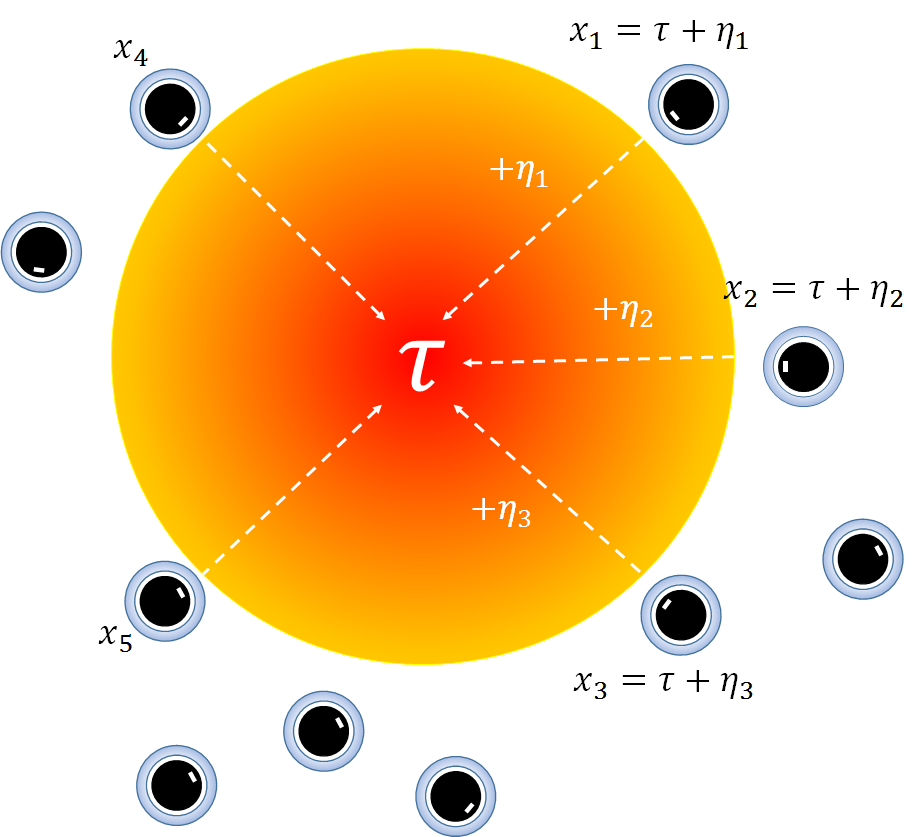
\includegraphics[width=0.4\textwidth]{figures/firefighting.png}
        \centering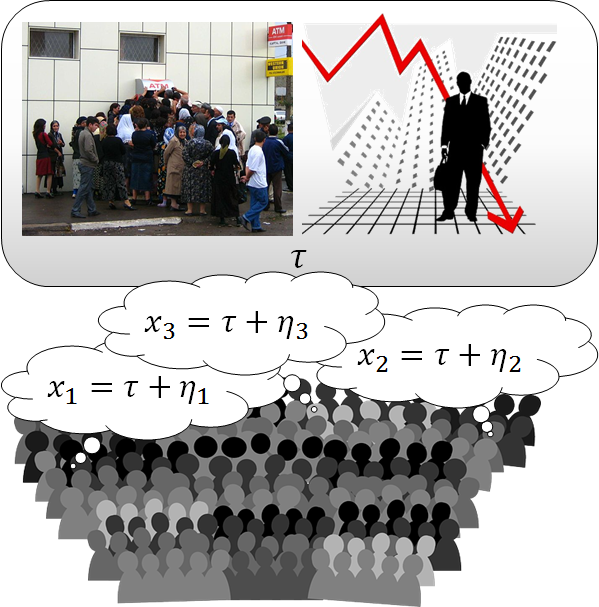
\includegraphics[width=0.4\textwidth]{figures/bankrun.png}
        \centering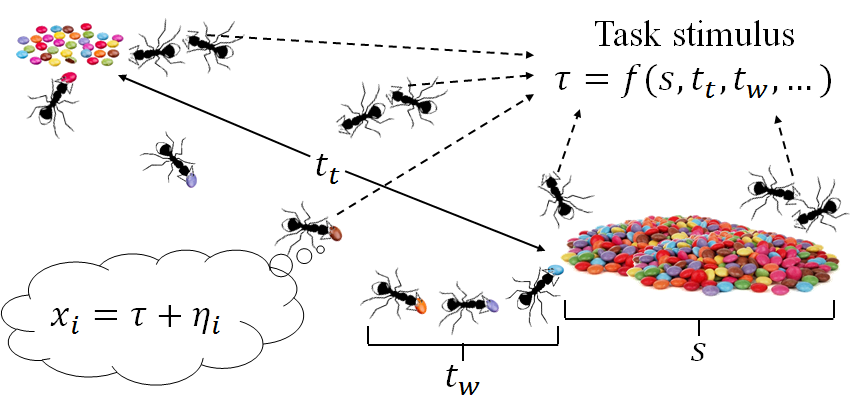
\includegraphics[width=0.8\textwidth]{figures/foraging.png}
    \caption{Robotic fire fighting, ant foraging, and bank run scenarios presented as global games. Each player's imperfect estimate of the task is represented by $x_i$, comprising of the global stimulus parameter $\tau$ and noisy sensor measurements $\eta_i$. In the robot firefighting scenario $\tau$ is representative of the magnitude of the fire, while in the case of a bank run $\tau$ is indicative of an agent's current level of trust in the nation's economy. For the ant foraging scenario $\tau$ represents an ant's willingness to take part in the foraging task based on a number of internally measured parameters such as the distance to the food source ($t_t$), the wait time to deliver food ($t_w$), and the food stores currently at the nest ($s$), among others.\label{fig:motivation}}    
\end{figure}


Situations like this arise in a number of different fields including neurology \citep{Yoshida2010,Suzuki2015}, ethology \citep{Robinson1987,Gordon1996,Bonabeau1998,Theraulaz1998}, sociology \citep{Raafat2009}, economics \citep{Morris2000}, and robotics \citep{Martinoli1999,Krieger2000,Kube2000,Pynadath2002,Gerkey2003, Mataric2003,Gerkey2004,Kanakia2014}. All of these multi-agent scenarios share the common notion of a joint action or response to a commonly observed stimulus. The task can take on many forms ranging from neurons simply firing in concert, collective decision problems like flocking, herd grazing and colony defense to individual actions based on the environment and other agents' beliefs like foraging, bank runs, and political revolutions. 

In the case of a bank run \citep{Morris2000}, $\tau$ is an aggregate stimulus parameter that represents the strength of the economy of a nation. Here, agents decide when to withdraw their assets from banks based on their own noisy estimate of the economy together with a simple threshold. In the case of social insects foraging for food \citep{Bonabeau1996,Theraulaz1998,Krieger2000}, $\tau$ represents a number of environmental cues such as the (imperfect) measurement of food stores in a colony, pheromone levels\citep{Robinson1987} or the waiting time for food transfer from one agent to another \citep{Seeley1989}.  A complex combination of these internal and external cues \citep{Gordon1996} temper an agent's perception of the magnitude of a task. In an engineering context, $\tau$ can be seen as the magnitude of a fire (heat intensity and area covered) as sensed by a robot using on-board instruments in an automated firefighting scenario \citep{Kanakia2014}. Figure \ref{fig:motivation} illustrates each of these three examples with their corresponding stimulus parameters. 

The group dynamic in the above examples may seem orthogonal at first; while adversarial behaviour between agents drives bank runs, collaborative behaviour between robots is essential for the automated firefighting scenario. Both scenarios, however, share the notion that to be successful an agent not only needs to assess the magnitude of the task itself but also the likelihood of the other agents to act. This is because only acting in concert leads to the desired group action, be it because using up water resources to put out a fire is futile before critical mass is reached, or disengaging from the banking system is non-desirable unless there is a major crisis. In a system with multiple tasks, such as an ant colony, coordination is required to achieve a desirable proportion between tasks.  

\subsection{Related work}
Task allocation is a canonical problem in multi-robot systems \citep{Gerkey2004}. Whereas capable robots might be able to approximate optimal task allocation, e.g., using market-based approaches \citep{Amstutz2008,Vig2007,choi2009consensus} or using  leader-follower coalition algorithms \citep{Chen2011}, probabilistic algorithms are of particular interest for swarm robotics with individually simple controllers \citep{Dantu2012} and little to no communication ability. Recruitment of an exact number of robots to a particular task has been extensively studied using the ``Stick Pulling'' experiment \citep{Lerman2001,Martinoli2004}. The problem of distributing a swarm of robots across a discrete number of sites/tasks with a specific desired distribution has been studied in \citep{Berman2009,Correll2008}. We showed in \citep{Kanakia2014} that these problems are related, as they can be cast as instances of sigmoidal threshold task allocation problems with varying slopes. Similarly, Mather \citep{Mather2010} presents a stochastic approach that is a hybrid between the work in \citep{Berman2009} and \citep{Martinoli2004}, allowing allocation to tasks requiring a varying number of robots. Yet, formally understanding probabilistic task allocation strategies is an open challenge. Although there exists differential equation models for specific classes of foraging problems \citep{lerman2006analysis,liu2010modelling} that allow to study the relationship between robot control parameters and resulting dynamics, results are purely phenomenological and leave it open as to whether there exist better or worse approaches for task allocation given the individual agent's capabilities. Other works address this question empirical, by performing comparisons of \edit{probabilistic} and deliberate strategies for certain classes of task allocation problems \citep{Kalra2006,correll2007coordination}. Here, the general insight is that stochastic task allocation is beneficial under the influence of noise, which leads to failure to optimal assignment techniques, thereby making them comparable with a stochastic strategy under such conditions. 

There exists also a rich body of work that uses techniques from game theory to multi-agent coordination \citep{parsons2002game,nisan2007algorithmic}, and task allocation in particular \citep{shehory1998methods}. While most works rely on the assumption of perfect information in the system, there is a branch of game theory in which information about characteristics of the other players is incomplete, which makes them applicable . These class of games are known as \emph{Bayesian games} \citep{harsanyi2004games} and are of particular interest to multi-agent systems problems that involve uncertainty. Here, \emph{global games} \citep{Carlsson1993} are a subset of Bayesian games, in which players receive possibly-correlated signals of the underlying state of the world, making them an interesting, but yet unexplored, avenue for modeling and understanding stimulus-response task allocation systems. 

\subsection{Contribution of this Paper}
This paper provides a formal analysis framework for threshold-based task allocation by formulating it as a ``Global Game'' (Section \ref{sec:globalgame}) and formally showing that a simple, communication-free threshold policy leads to a Baynesian Nash Equilibrium (Section \ref{sec:discretethreshold}). We then show that such a policy is equivalent to a sigmoidal threshold policy, which are commonly observed in social insects and used in swarm engineering, in Section \ref{sec:continuous}.

\section{Task Allocation as Global Games}\label{sec:globalgame}
We build on results from global games \citep{Carlsson1993} to show that the observed behaviour in all these scenarios can be effectively emulated by assuming that each agent makes their individual decision on whether or not to perform a task based on some internal threshold value which is compared to their noisy estimates of the collective task's stimulus $\tau$. This was shown for the canonical bank run example \citep{Morris2000}. While the classical global game assumes each agent must predict the other agents' behaviour, it turns out that agents can reach an equilibrium without this capacity. This, and the fact that agents do not need to communicate, makes this approach widely applicable to a wide range of multi-agent systems.

%We formalize the task allocation problem as a global game to mathematically prove the existence of BNE when a threshold based strategy is employed to solve the problem. 
Consider a set of $n$ agents and suppose that each agent has an action set $A_i=\{0,1\}$ where $0$ represents not participating in the task and $1$ represents participating in the task. Every agent is also aware of the total number of other agents, $n$ in the system. For the purpose of analysis we assume the decision to act or not to act is made by all agents at the same time, i.e.\ this is a one-shot game with no notion of time. We let the stimulus $\tau$ be a real number that belongs within the interval $E=[c,d]$ in $\R$. Finally, we let $u_i:A_i\times\Z^+\times \R\to \R$ be the utility of the $i^{\text{th}}$ agent, where $u_i(a_i,g,\tau)$ is the utility of the $i^{\text{th}}$ agent when $g$ other agents have decided to participate in the task. 
In general, the utility of each agent depends on the joint actions of the rest of the agents. For simplicity, we assume the utility to be proportional to the number of agents participating in the activity. %The following discussion can be substantially generalized but this form of utility serves the purpose of this study. 

The utility function discussed throughout this paper has the following properties:
\begin{enumerate}[a.]
	\item \edit{$u_i(1,g,\tau)-u_i(0,g,\tau)$ is an increasing and continuous function of $\tau$ for any $g$. We further assume that $|u_i(1,g,\tau)-u_i(0,g,\tau)|\leq \tau^p$ for some $p\geq 1$.}
	\item \edit{For extreme stimulus ranges, taking part in the activity is either appealing or repelling, i.e.\ there exists $\underline{\tau},\bar{\tau}\in (c,d)$ with $\underline{\tau}\leq \bar{\tau}$ such that for any $\tau\geq \bar{\tau}$ we have $u_i(1,g,\tau)>u_i(0,g,\tau)$ where all agents participate in very easy tasks, and for $\tau\leq \underline{\tau}$ we have $u_i(1,g,\tau)<u_i(0,g,\tau)$ so the only equilibrium of the game is for all agents to not participate as the task is too difficult.}
\end{enumerate}
Note that in order to have a task with such an utility, we need the above conditions to hold for all the agents, i.e.\ for all $i\in\{1,\ldots,n\}$. An example of a utility function that would satisfy such conditions is a function $u_i(a_i,g,\tau)=a_i(1-e^{-(g+1)}+\tau)$. 


The main challenge in devising task allocation strategies is that the true value of $\tau$ is not easily accessible to the agents, for example due to limited perception capabilities and sensor noise.
We model this imperfect knowledge by assuming that agent $i$ observes $x_i=\tau+\eta_i$ where $\eta_i$ is a Gaussian $\mathcal{N}(0,\sigma_i^2)$ random variable. Throughout our discussion, we assume that the task stimulus $\tau$ is a Gaussian random variable and is independent of $\eta_1,\ldots,\eta_n$. This analysis is extendable to a larger class of random variables but for the simplicity of the discussion, we consider Gaussian random variables here. Given these constraints, the question is what strategy the agents should follow to reach a BNE. In other words, an outcome in which no agent has the incentive to deviate from its current strategy.

A \emph{strategy} $s_i$ for the $i^{\text{th}}$ agent is a measurable function $s_i:\R\to A_i$, mapping measurements (observations) to actions. Strategy $s_i$ prescribes what action the $i^{\text{th}}$ agent should take given its own measurement $x_i$. Given this, consider a set of agents with strategies $s_1,\ldots,s_n$. Let us denote the strategies of the $n-1$ agents other than the $i^{\text{th}}$ agent by the vector $S_{-i}=\{s_1,\ldots,s_{i-1},s_{i+1},\ldots,s_n\}$.  We say that a strategy $s_i$ is a \emph{threshold strategy} if $s_i(x)=\text{step}(x, \td_i)$, i.e.\ the step function with a jump from $0$ to $1$ at $\td_i$, where $\td_i$ is the internal threshold value of the $i^{\text{th}}$ agent. For the $i^{\text{th}}$ agent, we define the best-response $BR(S_{-i})$ (to the strategies of the other agents) to be a strategy $\tilde{s}$ that for any $x\in \R$:

\begin{align*}\label{eqn:BR}
BR(S_{-i})(x)&=\tilde{s}(x)\in\amax{a_i\in A_i} E(u_i(a_i,g,\tau)\mid x_i=x)\\
&=\amax{a_i\in A_i} E(u_i(a_i,\sum_{j\not=i}s_j(x_j),\tau)\mid x_i=x),
\end{align*}
where $E(\cdot|\cdot)$ is the conditional expectation of $u_i$ given the $i^{\text{th}}$ agent's observation. \beh{The best response of player $i$ simply is the best course of action for agent $i$ given that the strategies of the other players is given. Indeed the expression $\amax{a_i\in A_i} E(u_i(a_i,g,\tau)\mid x_i=x)$ is the (set of) best actions that player $i$ can take given its information, the aggregate action $g$ of the other players, and the intensity $\tau$}. Note that given the $i^{\text{th}}$ agent's observation $x_i$, the observations of the other agents, and hence their actions, would be random from the $i^{\text{th}}$ agent perspective, i.e. given $x_i$ and $\tau$, all $s \in S_{-i}$ are effectively random variables with respect to the $i^{\text{th}}$ agent. A strategy profile $S=\{s_1,\ldots,s_n\}$ is a \emph{sensible strategy}, if it leads to a BNE \citep{Fudenberg1998}, given $s_i=BR(S_{-i})$ for all $i\in \{1,\ldots,n\}$. 

\section{Communication-free threshold-based Task Allocation Strategy}\label{sec:discretethreshold}
Any task with concurrent benefit admits a threshold strategy BNE---meaning it is sufficient for the agents to follow a simple algorithm: 
\begin{enumerate}[(i)]
\item Compare your noisy measurement $x_i$ to a threshold value $\td_i$,
\item If the measurement is above $\td_i$ take part in the collaborative task, otherwise hold off.
\end{enumerate}
This algorithm is extremely simple, and can be implemented on systems with a wide range of capabilities, yet leads to a BNE as we will show below.

To show that there exists a sensible threshold strategy for the class of tasks with concurrent benefit leading to Theorem 1, we will first show that the best response to threshold strategies is a threshold strategy (Lemma 1), and then show that there exists an equilibrium of threshold strategies \citep{Carlsson1993,Morris2000} (Lemma 2).

\setcounter{lemma}{0}

\begin{lemma}
Let $S=\{s_1,\ldots,s_n\}$ be a strategy profile consisting of threshold strategies for a task with  concurrent benefit. Let $\tilde{s}_i=BR(S_{-i})$. Then $\tilde{s}_i$ is a threshold strategy. 
\end{lemma} 

\begin{proof}
We first show that if for some observation $x_i=x$, we have $BR(S_{-i})(x)=\tilde{s}_i(x)=1$, then $\tilde{s}_i(y)=1$ for $y\geq x$. To show this,  we note that $P(x_j\geq \tau_j\mid x_i=x)$ is an increasing function of $x$ as $x_j-x_i$ is a normally distributed random variable. Therefore, using the monotone property of concurrent tasks and the fact that $x_i=\tau+\eta_i$, we conclude that:
\vspace{-5px}
\begin{align*}
&E(u_i(1,\sum_{j\not=i}s_j(x_j),\tau)\mid x_i=y)\\ 
&\qquad-E(u_i(0,\sum_{j\not=i}s_j(x_j),\tau)\mid x_i=y)\\ 
&>E(u_i(1,\sum_{j\not=i}s_j(x_j),\tau)\mid x_i=x)\\
&\qquad-E(u_i(0,\sum_{j\not=i}s_j(x_j),\tau)\mid x_i=x)\geq 0.
\end{align*}
Therefore $\tilde{s}_i(y)=1$. Similarly, if for some value of $x$, we have $\tilde{s}_i(x)=0$, then it follows that $\tilde{s}_i(y)=0$ for $y\leq x$. Therefore, $\tilde{s}_i$ would be a threshold strategy.  
\end{proof}

We can view the best-response of threshold strategies as a mapping from $\R^n$ to $\R^n$ that maps $n$ thresholds of the original strategies to $n$ thresholds of the best-response strategies. Denote this mapping by $L:\R^n\to\R^n$.
\begin{lemma}\label{lemma:continuous}
The mapping $L$ that maps the threshold values of threshold strategies to the threshold values of the best-response strategies is a continuous mapping. 
\end{lemma}


\begin{proof}
Let $x_{-i}=(x_1,\ldots,x_{i-1},x_{i+1},\ldots,x_n)$ be the vector of observations of $n-1$ agents except the $i^{\text{th}}$ agent. Note that the vector $(x_{-i},\tau)$ given $x_i=x$ is a normally distributed random vector with some continuous density function $f_{x}(x_{-i},\tau)$. Now, let $\{\alpha(k)\}$ be a sequence in $\R^n$ that is converging to $\alpha\in\R^n$. Let $\{\beta(k)\}$ be the sequence of thresholds corresponding to the best-response strategy of the strategy with threshold vector $\alpha(k)$. Let $s$ be the threshold strategy corresponding to the threshold vector $\alpha$ and let $\alpha^*$ be the threshold strategy corresponding to the $BR(\alpha)$. By the definition of the best-response strategy, $\beta_i(k)$ is a point where 
\begin{align*}
&\int_{\R^{n}}f_{\beta(k)}(z,t)\left(u_i(1,\sum_{j\not=i}u^{\alpha_j(k)}(x_j),\tau)\right.\\
&\qquad\left.-u_i(0,\sum_{j\not=i}u^{\alpha_j(k)}(x_j),\tau)\right)d(z\times t)=0.
\end{align*}
Using the fact that $f$ has a Gaussian distribution and is continuous on all its arguments and the fact that $|u_i(\cdot,\cdot,\tau)|\leq \tau^p$, by taking the limit $k\to\infty$ and the dominated convergence theorem:
\begin{align*}
&\int_{\R^{n}}f_{\beta}(z,t)(u_i(1,\sum_{j\not=i}u^{\alpha_j}(x_j),\tau)\\ 
&\qquad-u_i(0,\sum_{j\not=i}u^{\alpha(k)}(x_j),\tau))d(z\times t)=0,
\end{align*}
where $u^{r}$ is a threshold strategy with threshold $r$. Therefore, the $\lim_{k\to\infty}L(\alpha(k))=L(\alpha)$ for a sequence $\{\alpha(k)\}$ that is converging to $\alpha$.
\end{proof}

Using these lemmas, we can show the existence of a threshold strategy for global games with concurrent benefit. 
\begin{theorem}\label{thrm:mainthrm}
For a concurrent benefit task $T$, suppose that the stimulus parameter $\tau$ is a Gaussian random variable. Also, suppose that $x_i=\tau+\eta_i$ where $\eta_1,\ldots,\eta_n$ are independent Gaussian random variables. Then, there exists a strategy profile $S=(s_1,\ldots,s_n)$ of threshold strategies that is a BNE.
\end{theorem}
\begin{proof}
By Lemma 1, the best response of a threshold strategy is a threshold strategy and hence, it induces the mapping $L$ from the space of thresholds $\R^n$ to itself. Also, by Lemma~\ref{lemma:continuous}, this mapping is a continuous mapping. Now, if $\td_i$ is a sufficiently large threshold, then the second property of concurrent benefit tasks implies that the $\tilde{\td}_i\leq \td_i$ because a large enough measurement $x_i$ implies that agent $i$ itself should take part in the task. Similarly, for sufficiently low threshold $\td_i$, we will have $\tilde{\td}_i\geq \td_i$. Therefore, the mapping $L$ maps a box $[a,b]^n$ to itself, where $a$ is a sufficiently small scalar and $b>a$ is a sufficiently large scalar. Since the box $[a,b]^n$ is a convex closed set, by the Brouwer's fix point theorem \citep{Border1990} we have that there exists a vector of threshold values $\alpha^*$ such that $\alpha^*=L(\alpha^*)$ and hence, there exists a BNE for the concurrent benefit task $T$.
\end{proof}

\section{From discrete thresholds to sigmoidal response functions}\label{sec:continuous}
Observations in ethology suggest sigmoid threshold functions \citep{Bonabeau1996}, rather than fixed thresholds as suggested by our analysis. Also, roboticists have started using sigmoid-shaped threshold functions to engineer swarm systems \citep{Bonabeau1996,Theraulaz1998,Krieger2000}, as tuning the shape of a sigmoidal response threshold function allows balancing between exploration, i.e., performing a random action, and exploitation, i.e., using all available information in decision making such as a fixed threshold. 
We argue that this behavior can be a direct result of using a simple discrete threshold under the influence of perception noise. Indeed, one can show that a sigmoid threshold function is the outcome of deterministic threshold functions on noisy observations. Suppose that all  agents share the same utility function $u(a_i,g,\tau)$ and also, assume that the observation noise of the $n$ agents ($\eta_1,\ldots,\eta_n$) are independent and identically distributed (IID) $\mathcal{N}(0,\sigma^2)$ Gaussian random variables. Then, it is not hard to see that there exists a BNE with threshold strategies that have the same threshold value $\td$ \citep{Morris2000}.

Consider a realization of $\tau=\hat{\tau}$ and suppose that we have a large number of agents $n$ observing a noisy variation of $\hat{\tau}$. Take for example the case of fire-fighting agents, and let $\hat{\tau}$ be the magnitude (including type, intensity, area, etc.) of the fire. Then, since the observations of the $n$ agents are IID given the value of $\tau$, they will be distributed according to $\mathcal{N}(\hat{\tau},\sigma^2)$. Now consider the relative number of agents taking part in the activity given $\hat{\tau}$ as defined by,

\begin{equation*}
	N_{rel}(\hat{\tau}):=\frac{\#\text{agents with }x_i\geq \td}{n}.
\end{equation*}
We can now show that for the relative number of agents $N_{rel}(\hat{\tau})$, we have
\begin{equation}
\lim_{n\to\infty}N_{rel}(\hat{\tau})=\Phi(\frac{\hat{\tau}-\td}{\sigma^2})
\end{equation}
where $\Phi$ is the cumulative distribution function (cdf) of a standard Gaussian, which is illustrated numerically in Figure 2, and shown in Theorem 2:  

\begin{theorem}\label{thrm:relativefrequency}
For the relative number of agents $N_{rel}(\hat{\tau})$, we have
\begin{equation}
\lim_{n\to\infty}N_{rel}(\hat{\tau})=\Phi(\frac{\hat{\tau}-\td}{\sigma^2})
\end{equation}
where $\Phi$ is the cumulative distribution function (cdf) of a standard Gaussian. 
\end{theorem}
\begin{proof}
Note that $N_{rel}(\hat{\tau})=\frac{\sum_{i=1}^n\mathbf{I}_{x_i\geq \td}}{n}$ where $\mathbf{I}_{i\geq j}$ is the indicator function for $i\geq j$. For a given $\hat{\tau}$, $x_i$ are IID $\mathcal{N}(\hat{\tau},\sigma^2)$ random variables and hence, $\mathbf{I}_{x_i\geq \td}$ are IID random variables for all agents with $E(\mathbf{I}_{x_i\geq \td})=\Phi(\frac{\hat{\tau}-\td}{\sigma^2})$. Therefore, by the Law of Large Numbers, it follows that:
\begin{align*}
\lim_{n\to\infty}N_{rel}(\hat{\tau})=\Phi(\frac{\hat{\tau}-\td}{\sigma^2}).
\end{align*}
\end{proof}

The final step to explain the prevalence of sigmoid functions in multi-agent settings is to note that:

\vspace{-20px}
\begin{align*}
|\Phi(\frac{\hat{\tau}-\td}{\sigma^2})-\frac{1}{1+e^{-d(\frac{\hat{\tau}-\td}{\sigma^2})}}|\leq 0.01,
\end{align*}
for all $\hat{\tau}\in\R$ and some optimal value $d\approx 1.704$ as described in \citep{Camilli1994}. This means that the aggregate behavior of the agents following deterministic threshold strategies would closely follow (to within a constant error term) the shape of the commonly observed logistic sigmoid function whose drift is directly proportional to $\td$ and the slope is inversely proportional to $\sigma^2$. 

Therefore, despite agents using deterministic threshold strategies, their \emph{aggregate behavior} would appear to an outside observer as a continuous sigmoid threshold function instead of numerous discrete thresholds.
\begin{figure}[!ht]
	\centering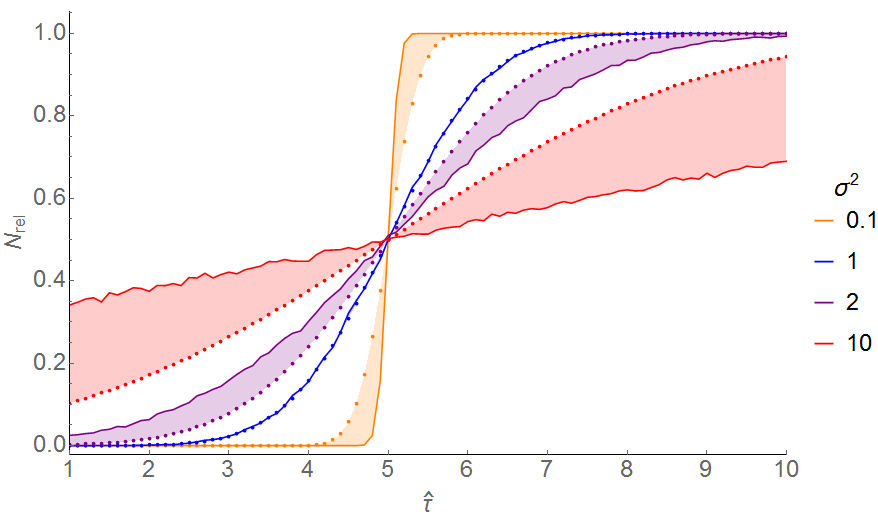
\includegraphics[width=0.6\columnwidth]{figures/thm2fig.png}
	\centering\caption{Visualization of Theorem~2 as $N_{rel}$ estimates $\Phi(\cdot)$. The plot was generated by running Eqn.~1 10,000 times for each point in $\hat{\tau} = 1$ to $10$ in increments of $0.1$. $n = 10$, $\td = 5$ and $x_i = \hat{\tau} + \eta_i$ ($\eta_i \sim\mathcal{N}(0, \sigma^2)$). Each curve in the plot is generated by sweeping $\sigma^2 = \{0, 0.1, 1, 2, 10\}$, with $\sigma^2 = 0$ being a step-function and $\sigma^2 = 10$ having the \emph{flattest} slope.}\label{fig:thm2fig}
\end{figure}

\section{Discussion}
Although we have shown how a simple threshold based policy for task allocation leads to a BNE and can resemble behavior observed in social insects, we caution that all proofs in this paper assume Gaussian distributions for the stimulus parameter and its observations. While these assumptions can easily be accomodated in an engineering context, they do not necessarily hold for biologicalical context. Studying the true distributions in systems of interest and extending the results presented here for other distributions is therefore subject to further work. 

We also note that the proposed task allocation mechanism is not optimal in terms of the allocations it can generate, but simply the best strategy for an individual agent given that other agents are using the same policy, which is the definition of a Nash equilibrium. This strategy is therefore only interesting if communication between agents is impossible or otherwise too costly. In this case, the proposed framework offers an analysis framework, which makes such an approach viable in an engineering context. Yet, further work is needed to formally show what the lower performance bounds of such a policy are. 



\section{Conclusion}
Results presented in this paper suggest that global games can  describe a wide range of collective decision making scenarios, explaining the prevalence of sigmoid threshold strategies in natural and artificial systems. By varying noise in the system and thereby changing the slope of the sigmoid function, the response threshold strategy also allows the system to balance between exploitation and exploration. This, in turn, may lead to designing robust robot swarms that are flexible and can alter strategies for changing environmental parameters without requiring communication; a highly desired property that is often observed in natural swarms and is of great interest for engineered systems.

%\nolinenumbers
\section*{Acknowledgments}
A. Kanakia and N. Correll have been supported by NSF CAREER grant \#1150223. We are grateful for this support.

\bibliographystyle{agsm}
\bibliography{refworks}



% For your review copy (i.e., the file you initially send in for
% evaluation), you can use the {figure} environment and the
% \includegraphics command to stream your figures into the text, placing
% all figures at the end.  For the final, revised manuscript for
% acceptance and production, however, PostScript or other graphics
% should not be streamed into your compliled file.  Instead, set
% captions as simple paragraphs (with a \noindent tag), setting them
% off from the rest of the text with a \clearpage as shown  below, and
% submit figures as separate files according to the Art Department's
% instructions.






\end{document}




















